%-------------------------------%
%  Author: Alessandro Sciarra   %
%    Date: 19 Oct 2020          %
%-------------------------------%

%~~~~~~~~~~~~~~~~~~~~~~~~~~~~~~~~~~~~~~~~~~~~%
\begingroup
\newsavebox{\shUnitLink}
\begin{frame}{One slide about testing: The tests pyramid}
    \savebox{\shUnitLink}{\URL[PB]{https://github.com/kward/shunit2}{Shell unit test framework}}
    \begin{center}
        \resizebox{!}{0.8\textheight}{
            \begin{tikzpicture}
                \path coordinate (A) at (0,0)
                      coordinate (B) at (0,2)
                      coordinate (C) at (0,4)
                      coordinate (D) at (0,6)
                      coordinate (O) at ($(A)+(150:5)-(0.5,0)$);
                \draw (O) -- ++(30:5); %Just draw axis behind pyramid
                \begin{scope}[scope on=<6>]
                    \draw (A) ++(0,0.75) -- ++(30:5) -- ++(0.75,0) node[right] {\usebox{\shUnitLink}};
                    \draw (D) ++(0,0.75) -- ++(30:2) -- ++(0.75,0) node[right, text=PP] {Usually not so tough to be written in Bash};
                \end{scope}
                %Draw Pyramid
                \uncover<2->{\pyramidLayer{A}{1.5}{5}{red}{Unit};}
                \uncover<3->{\pyramidLayer{B}{1.5}{4}{orange!80!yellow}{Integration};}
                \uncover<4->{\pyramidLayer{C}{1.5}{3}{PS}{System};}
                \uncover<5->{\pyramidLayer{D}{1.5}{2}{PP}{Acceptance};}
                \draw[to] (O) -- ++(0,6) node[right, anchor=north west] {
                    \begin{tabular}{l}
                        Development cost\\
                        Execution time
                    \end{tabular}};
                \draw[to] (O) -- ++(330:6) node[right] {Number of tests};

            \end{tikzpicture}
        }
    \end{center}
    \PrepareURLsymbol[PB]
    \FrameRemark<5-6>{If you want to know more about this subject, also more in general, refer \URL*{https://github.com/AxelKrypton/Clean-code-good-practices}{to the second of these presentations}.}
\end{frame}
\endgroup
%~~~~~~~~~~~~~~~~~~~~~~~~~~~~~~~~~~~~~~~~~~~~%
\begin{frame}{My script does not do what it should: What can I do?}
    \begin{overlayarea}{\textwidth}{0.7\textheight}
        \begin{enumerate}
            \item Trying to debug it by hand is always a possibility\ldots \Remark{if you do so, try to do it in a clever way}
            \item<2-> \ldots{}alternatively you can run \URL[PB]{https://github.com/koalaman/shellcheck}{ShellCheck} on it or \URL[PB]{https://www.shellcheck.net}{use it online}!
        \end{enumerate}
        \begin{varblock}{}[\textwidth]{ShellCheck}<only@3>
            ShellCheck is a GPLv3 tool that gives warnings and suggestions for Bash/sh shell scripts:\\[0.3em]
            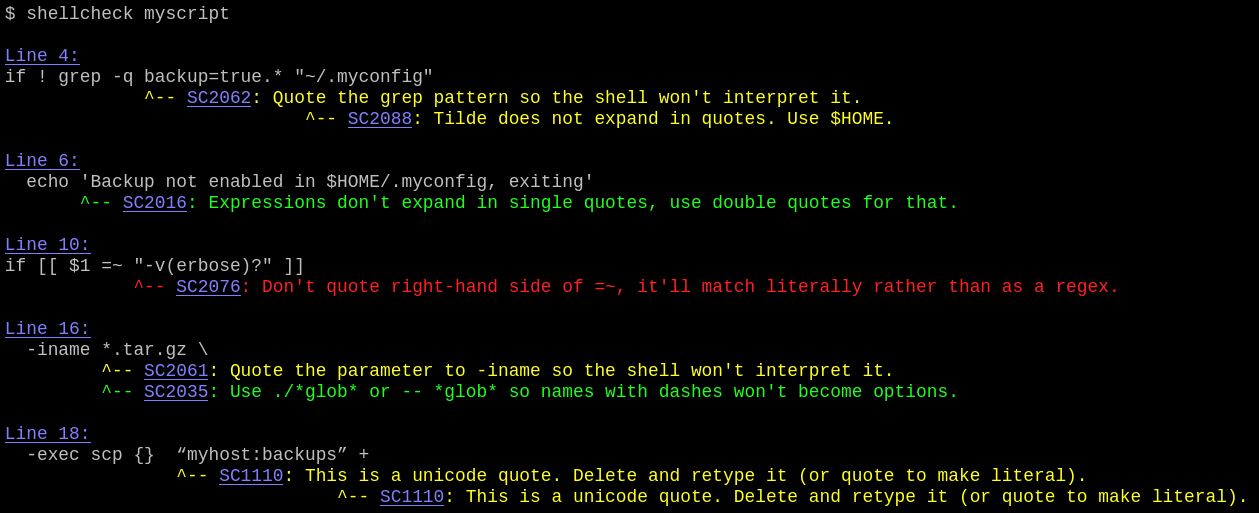
\includegraphics{ShellCheckExample}
        \end{varblock}
        \begin{varblock*}{example}[0.9\textwidth]{The goals of ShellCheck are}<only@4>
            \begin{itemize}
                \item To point out and clarify \PP{typical beginner's syntax issues} that cause a shell to give cryptic error messages.
                \item To point out and clarify \PB{typical intermediate level semantic problems} that cause a shell to behave strangely and counter-intuitively.
                \item To point out \alert{subtle caveats, corner cases and pitfalls} that may cause an advanced user's otherwise working script to fail under future circumstances.
            \end{itemize}
        \end{varblock*}
        \begin{itemize}[<only@4>]
            \item You can enable it on the fly in your editor
            \item You can ignore specific warnings/errors using directives
            \item Every implemented rule has a dedicated Wiki-page
                  \Remark{e.g. \URL[PB]{https://github.com/koalaman/shellcheck/wiki/SC1000}{https://github.com/koalaman/shellcheck/wiki/SC1000}}
        \end{itemize}
    \end{overlayarea}
\end{frame}
